\chapter{Simulación con Webots} \label{cap:simulación_con_webots}
% BREVE DESCRIPCIÓN DEL CONTENIDO DE ESTE CAPÍTULO
Webots es el simulador utilizado en el resto de este trabajo para mostrar el funcionamiento de los diferentes algoritmos desarrollados, este capítulo expone sus cualidades. En la sección \ref{sec:conceptos_básicos_del_simulador_Webots}, se describen las principales características que posee, los lenguajes y plataformas compatibles con el software. También, se definen conceptos esenciales para el desarrollo con el simulador como: mundo, controladores y controladores supervisores. La sección \ref{sec:el_formato_open_street_maps} explica la forma de integrar el formato \textit{Open Street Maps} con Webots en la búsqueda de crear escenarios de prueba más realistas. Por otro lado, la sección \ref{sec:el_ambiente_de_simulación} presenta las necesidades requeridas en este proyecto, se listan las características del ambiente simulado y del vehículo de pruebas, a continuación, se muestran los modelos finales del vehículo y escenario de pruebas. La sección \ref{sec:contribuciones_en_el_TMR} da a conocer las contribuciones de este trabajo en el TMR-AutoModelCar 2022.


\section{Conceptos básicos del simulador Webots} \label{sec:conceptos_básicos_del_simulador_Webots}

Webots es un software multiplataforma de código abierto enfocado a simulación de robots móviles, el ambiente de Webots provee un entorno de desarrollo completo que facilita la programación, modelado y simulación de robots de manera profesional. También, le permite al usuario crear entornos virtuales 3D con propiedades físicas importantes en el comportamiento de robots, tal es el caso de propiedades como: masa, coeficiente de fricción, articulaciones, entre otros\cite{Webots}.

En el simulador se pueden encontrar objetos pasivos y activos también llamados robots móviles, estos pueden ser equipados con una gran variedad de sensores y actuadores que contiene el propio simulador, donde destacan: sensores de distancia, sensores láser, motores, cámaras, ruedas, gps, emisores y receptores. Además ofrece al usuario la facilidad de programar de manera individual cada robot creado con el fin de lograr el comportamiento deseado para cada uno. La figura \ref{fig:webots_ui} ilustra la interfaz de usuario de Webots.
\begin{figure}
    \centering
    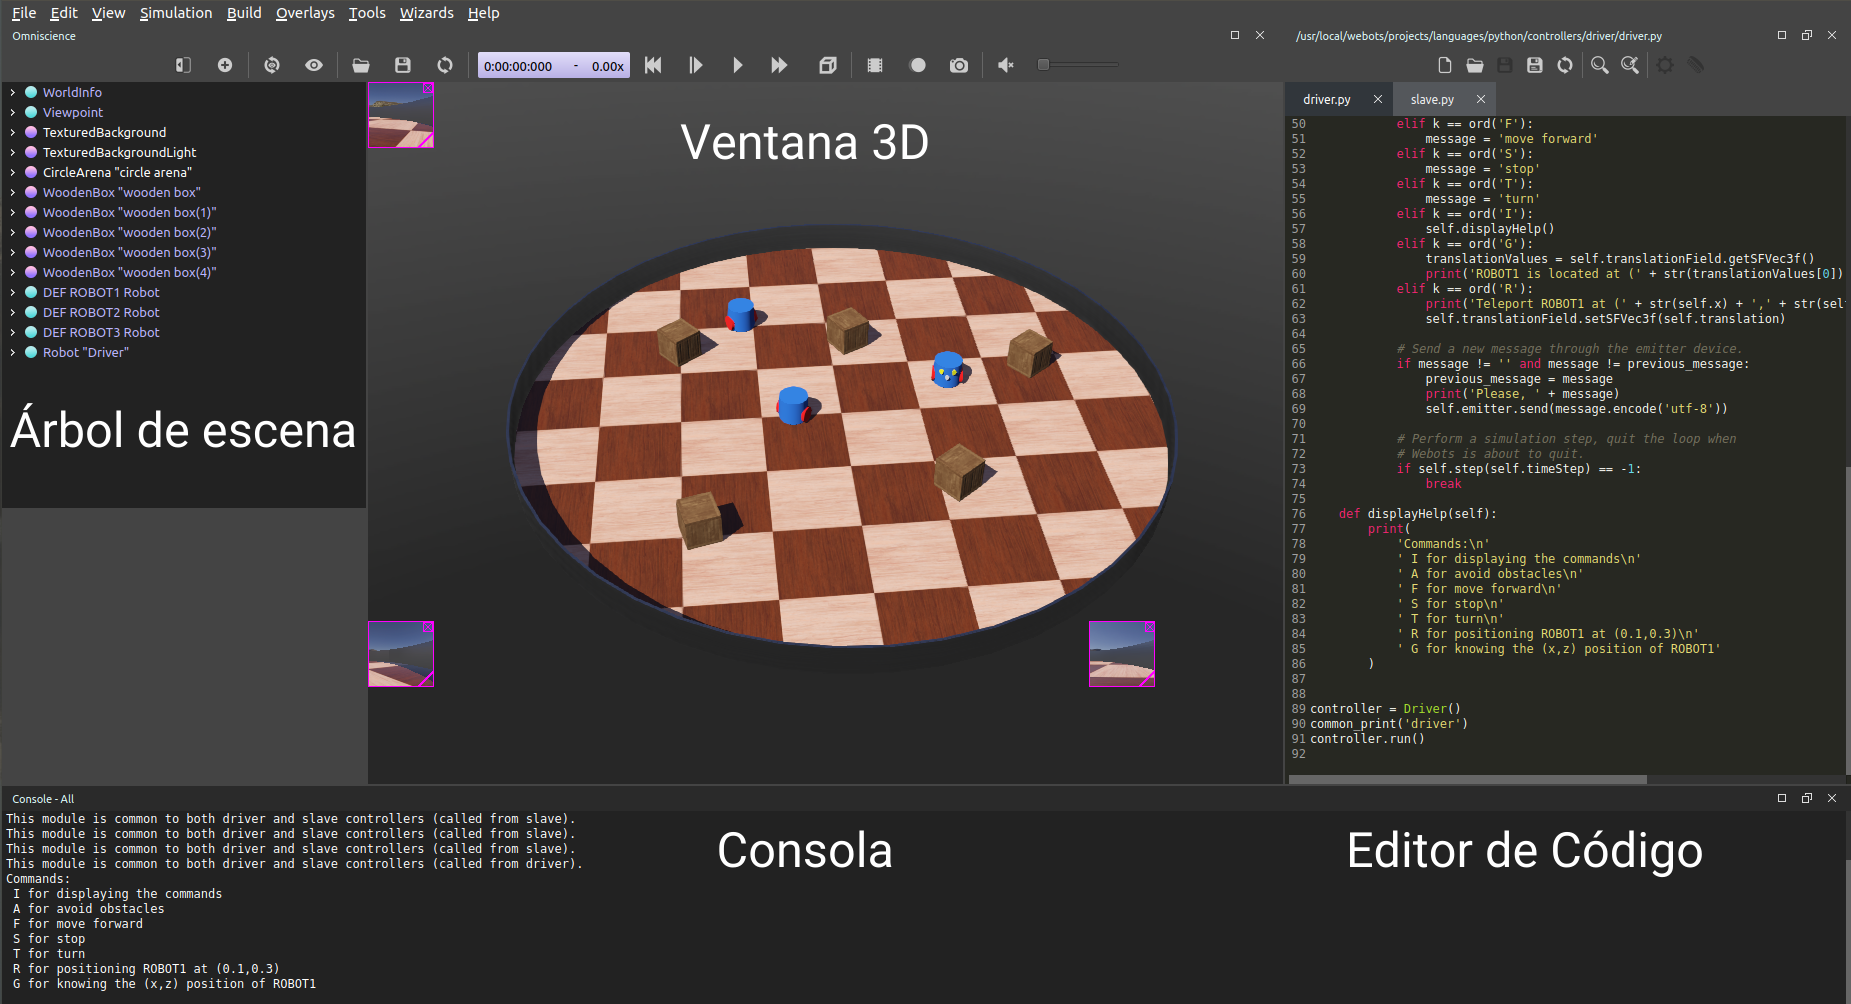
\includegraphics[width=0.5\textwidth]{Figures/Figures_Cap03/WebotsUserInterface.png}
    \caption{Interfaz de Usuario Webots.}
    \label{fig:webots_ui}
\end{figure}

\subsection{Lenguajes y Sistemas Operativos}

Al ser un software de código abierto Webots puede ser utilizado en diferentes plataformas de escritorio como: Windows, Linux y macOS. Para cada una de estas plataformas se encuentra disponible la documentación correspondiente, además existe una comunidad muy activa en cada una de sus variantes. Sin embargo, las distribuciones Linux son las que se mayor ayuda proveen, esto debido a la amplia compatibilidad entre Webots y las diferentes herramientas en el desarrollo de robots móviles. Por otra parte, Webots cuenta con soporte para diferentes lenguajes de programación en la creación de programas controladores, entre los lenguajes soportados se encuentran lenguajes compilados como: C, C++ y Java, también permite el uso de lenguajes interpretados como: Python y MATLAB\cite{Webots}.

\subsection{Controladores, supervisores y mundos} 

Para crear una simulación en Webots son necesarios dos elementos principales: un mundo y uno o varios controladores.

\begin{itemize}
    \item \textbf{Mundo:} En Webots un mundo es el conjunto de elementos que unido al robot forman una escena 3D o abstracción del mundo real con el fin de simular un ambiente real. Un mundo específica la descripción de cada objeto mediante propiedades como: posición, geometría, orientación, apariencia y propiedades físicas (en caso de ser necesarias). Cada objeto definido puede contener a su vez otro objeto diferente\cite{Webots}. En la figura \ref{fig:webots_example}, se observa un mundo de ejemplo creado en Webots. 
    %un mundo es una representación del ambiente mediante la descripción en 3D de las propiedades de el robot y el entorno en el que se encuentra, es decir, 
    
    \item \textbf{Controlador:} Es un programa que permite ejecutar acciones de control para un robot específico en un mundo específico. Dichos controladores pueden ser desarrollados en los diferentes lenguajes de programación soportados(C, C++, Java, Python, MATLAB). Para cada uno de estos lenguajes se provee la documentación necesaria. Una característica importante de los controladores es que un controlador puede ser utilizado por diferentes robots pero un robot solo puede usar un controlador. Al iniciar una simulación Webots lanza los controladores previamente asignados en cada robot, es decir, para cada controlador existe un proceso independiente\cite{Webots}.
    
    \item \textbf{Controlador Supervisor:} Este tipo de controladores son una variante especial de los controladores tradicionales, la principal diferencia entre ellos es que los controladores supervisores tienen acceso a operaciones privilegiadas. Por ejemplo; el control de simulación para mover el robot a una posición aleatoria, realizar una captura de vídeo de la simulación, entre otras. Los supervisores también pueden ser escritos en los lenguajes soportados por Webots\cite{Webots}.
\end{itemize}

\begin{figure}[h]
    \centering
    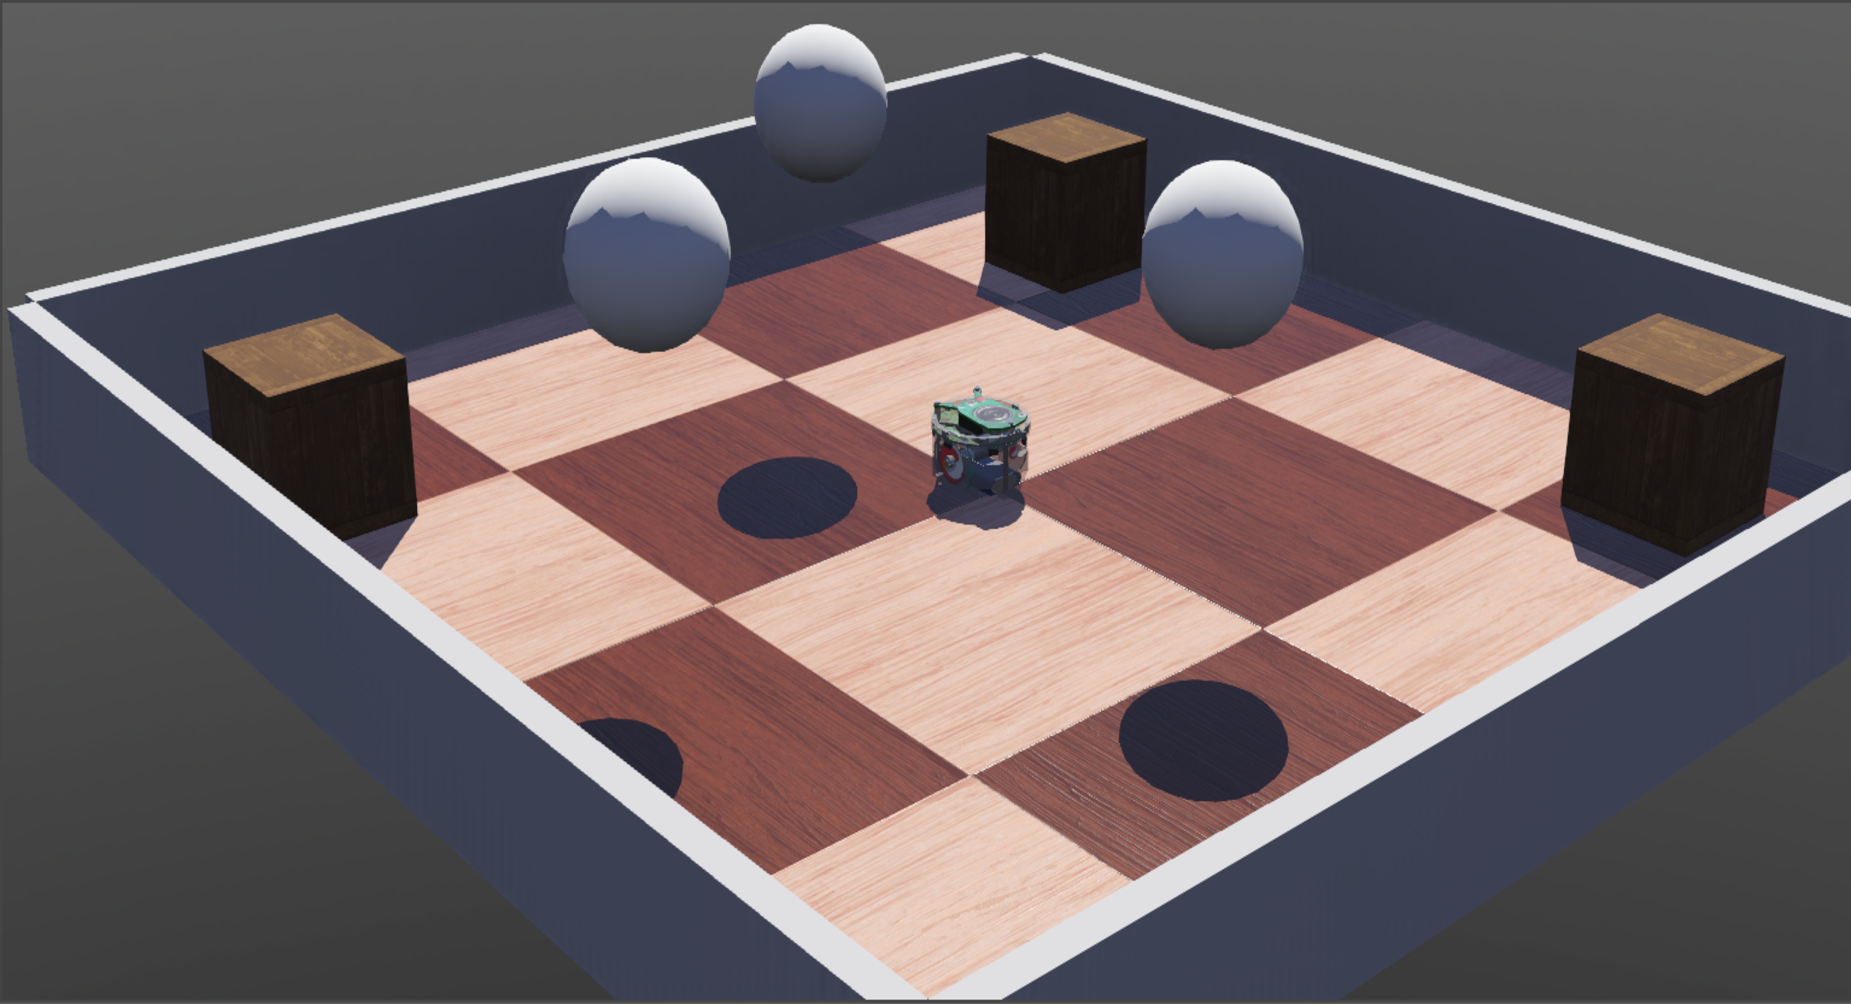
\includegraphics[width=0.5\textwidth]{Figures/Figures_Cap03/WebotsWorldExample.png}
    \caption{Ejemplo de mundo en Webots.}
    \label{fig:webots_example}
\end{figure}

%\textcolor{red}{
%\begin{itemize}
%\item Lenguajes y sistemas operativos soportados
%\item Controladores, mundos y controladores supervisores.
%\end{itemize}
%}

\section{El formato \textit{Open Street Maps}} \label{sec:el_formato_open_street_maps}

\subsection{Características y especificaciones}

El formato \textit{Open Street Maps} es un proyecto de software libre, global y cooperativo para la creación de mapas en base a información geográfica capturada por dispositivos GPS y ortofotografías, al ser un proyecto libre se cuenta con grandes cantidades de información y representación de mapas de casi cualquier sitio del mundo. Con base en el formato \textit{OSM} Webots es capaz de transformar la información del mapa en un ambiente 3D donde los principales objetos son las carreteras, conexiones viales y edificios. Además, mediante la integración de nodos específicos como: vehículos, señales de tránsito, obstáculos y mobiliario urbano se obtiene un ambiente de simulación (mundo 3D) con mayor detalle para el desarrollo de pruebas en conducción autónoma.

\subsection{Como usarlo en Webots}

Con el fin de implementar tareas de vehículos autónomos se requiere de un ambiente de simulación que cuente con las características necesarias y que sean lo más parecidas a un ambiente del mundo real. Para lidiar con este aspecto Webots ofrece una herramienta muy útil, la cual es generar modelos 3D a partir de una sección del mundo real tomada del formato \textit{Open Street Maps}. La manera de integrar OSM con Webots es muy sencilla debido a que desde la instalación inicial del simulador se incluyen las herramientas necesarias. En breve se enuncian los pasos a seguir para crear un escenario 3D inspirado en un mapa real.
\begin{figure}
        \centering
        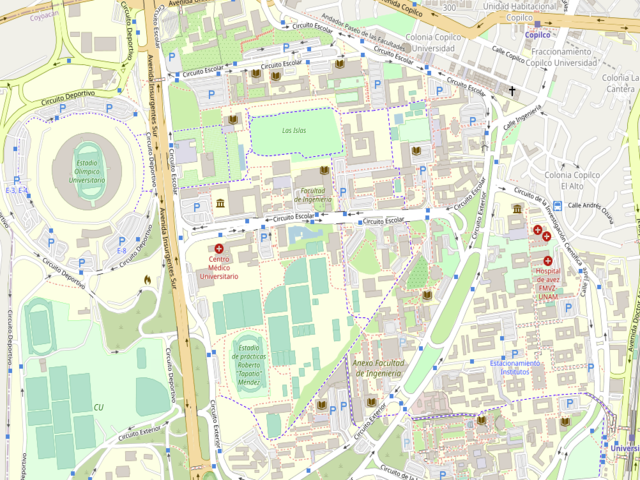
\includegraphics[width=0.5\textwidth]{Figures/Figures_Cap03/cu_osm.png}
        \caption{Sección de mapa obtenida de \textit{Open Street Maps}.}
        \label{fig:cu_osm}
\end{figure}

\begin{enumerate}
    \item Crear un directorio donde se alojará el proyecto.
    \item Obtener y descargar el mapa en formato OSM desde la página oficial de \textit{OpenStreetMap} \ref{fig:cu_osm} para generar el mundo de Webots.  
    %Desde la página web de OpenStreetMap se cuenta con la opciones para buscar y obtener una sección específica del mapa, en se aprecia una sección de mapa en Open Street Maps.
    
    \item Generar el mundo de Webots a partir del mapa obtenido. Webots cuenta con script ``importer.py'' que recibe como parámetro un archivo con extensión ``.osm'' y retorna como salida un archivo con extensión ``.wbt''. Es necesario ejecutar el script ``importer.py'' asignando como entrada el mapa previamente obtenido. Si la operación es exitosa se debe localizar un archivo ``.wbt'' en el directorio creado al inicio. Desde Webots se puede abrir el archivo para su visualización.
    
    \item Entrar a Webots y editar las carreteras, caminos y nombres de los mismos con el fin de eliminar cualquier \textit{bug} producido por ``importer.py'' debido a la complejidad del archivo ``.osm''. En esta etapa se pueden agregar más objetos (autos, árboles, señales, edificios, obstáculos) según sean requeridos. La figura \ref{fig:cu_wbt} muestra el resultado esperado de este proceso.
\end{enumerate}
\begin{figure}[h]
    \centering
    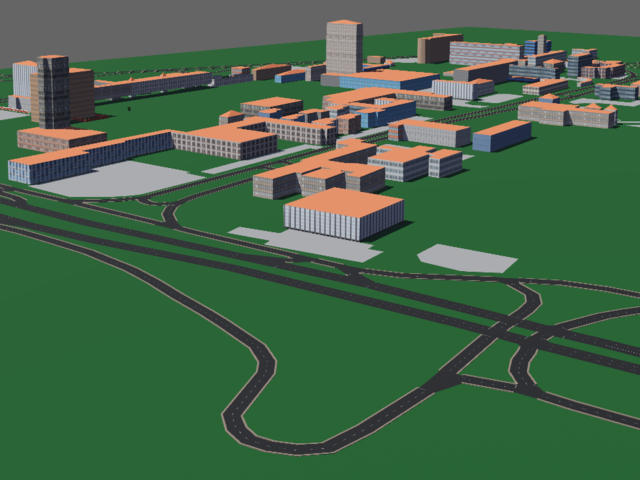
\includegraphics[width=0.45\textwidth]{Figures/Figures_Cap03/cu_wbt.png}
    \caption{Mundo de Webots generado a partir de una sección de mapa en formato ``.osm''.}
    \label{fig:cu_wbt}
\end{figure}


%\textcolor{red}{
%\begin{itemize}
%\item características y especs
%\item Cómo usarlo con Webots
%\end{itemize}
%}

\section{El ambiente de simulación} \label{sec:el_ambiente_de_simulación}

En la búsqueda de modelar comportamientos de vehículos autónomos reales como: detección y seguimiento de carriles, seguimiento de vehículos, detección y evasión de obstáculos tanto estáticos como dinámicos, es de vital importancia tener un escenario los más parecido posible a un ambiente vial cotidiano. Un ambiente vehicular tradicional es aquel que cuenta con automóviles en movimiento y estáticos, señales de tránsito, semáforos, carriles con dirección y espacios definidos. Además de contar con construcciones como edificios, casas, puentes e incluso personas y animales. Cada uno de estos elementos en conjunto forman un ecosistema vial como cualquier otro presente en localidades urbanas.

En este trabajo se pretende modelar un escenario 3D con el simulador Webots que integre las características suficientes para realizar ejercicios de prueba de diferentes comportamientos como:
\begin{itemize}
    \item Detección de Carril
    \item Seguimiento de Carril
    \item Detección de Obstáculos
    \item Evasión de Obstáculos
    \item Seguimiento de vehículos
    \item Acciones de rebase
\end{itemize}

Además de modelar un escenario con los elementos correspondientes se necesita de un vehículo (modelado en 3D) instrumentado con sensores y actuadores suficientes para cumplir tales comportamientos, ejemplos de sensores para instrumentación son:
\begin{itemize}
    \item Cámaras estéreo, RGB, RGD-D
    \item LIDAR
    \item RADAR
    \item GPS
    \item Giroscopio
\end{itemize}
%El elemento principal del escenario es el piso, pues es el lugar donde se encuentran situados los elementos restantes para un ambiente urbano,

Teniendo en cuenta las características descritas anteriormente se decide crear un escenario que satisfaga las necesidades solicitadas. Dentro de estos elementos se encuentra la carretera como un circuito cerrado. Al ser un circuito cerrado se tienen curvas y rectas, estas son pruebas muy comunes para cualquier vehículo ya sea tripulado o autónomo. La distribución de la carretera se compone de dos carriles en un solo sentido, esta distribución de espacio permite modelar el movimiento de otros vehículos, cada carril cuenta con líneas que delimitan el espacio asignado. Especialmente  estas líneas ayudan a completar las tareas de detección y seguimiento de carril pues funcionan como guía para el vehículo. La figura \ref{fig:world_lanes} ejemplifica los carriles de la carretera modelada.
\begin{figure}
    \centering
    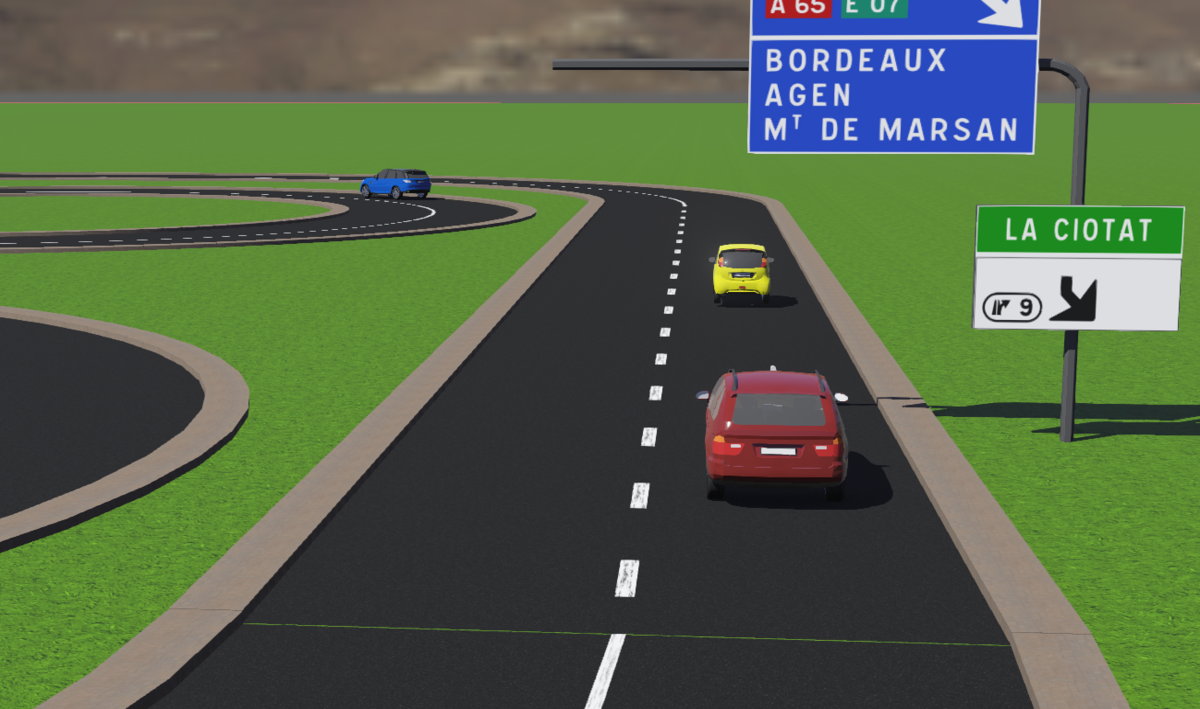
\includegraphics[width=0.5\textwidth]{Figures/Figures_Cap03/world_lanes.png}
    \caption{Carriles de la carretera.}
    \label{fig:world_lanes}
\end{figure}
Con la adición de otros vehículos dentro de la carretera se busca realizar detección y evasión de obstáculos, seguimiento y rebase de vehículos. El conjunto de estos objetos más otros elementos como: bordes en la carretera, áreas verdes e iluminación forman el escenario final donde se realizarán pruebas de conducción autónoma. Algunos elementos como: personas, mobiliario urbano, edificios, puentes, señales de tránsito y viales no se agregan al escenario ya que no resultan necesarias para este trabajo. El escenario final es el mostrado en \ref{fig:webots_world}.
\begin{figure}[h]
    \centering
    \begin{subfigure}[b]{0.4\textwidth}
         \centering
         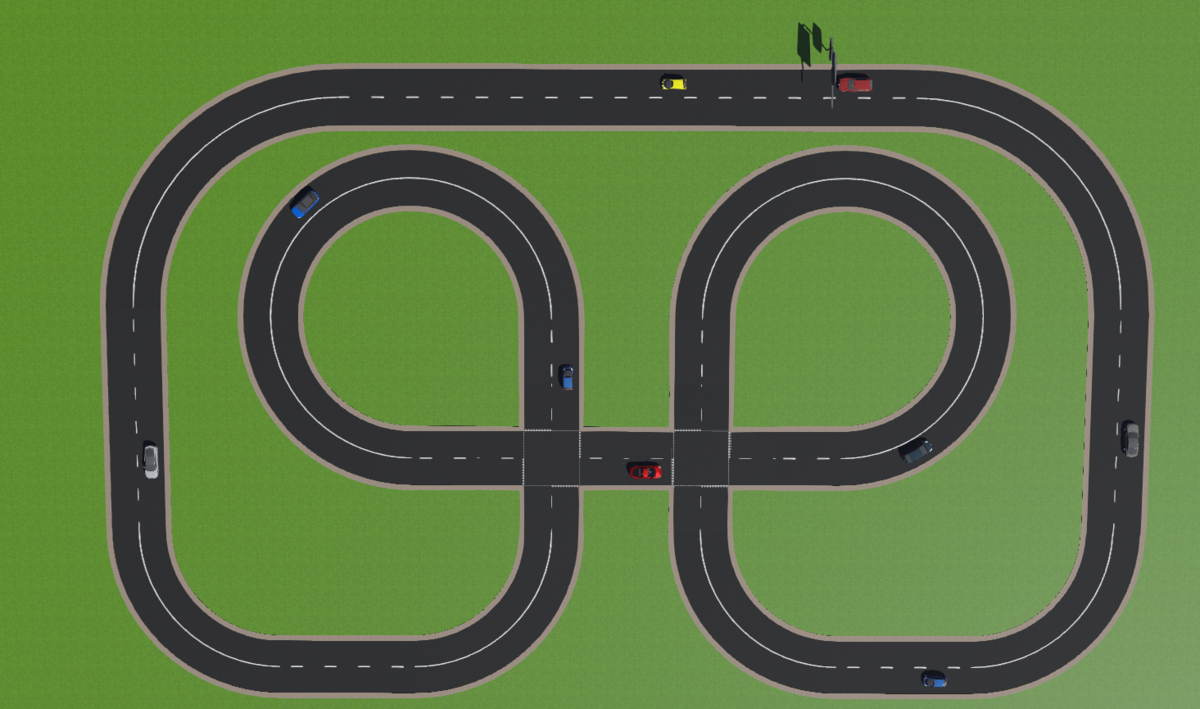
\includegraphics[width=\textwidth]{Figures/Figures_Cap03/webots_world.png}
         \caption{Escenario de pruebas de navegación.}
         \label{fig:webots_world}
    \end{subfigure}
    \hfill
    \begin{subfigure}[b]{0.375\textwidth}
         \centering
         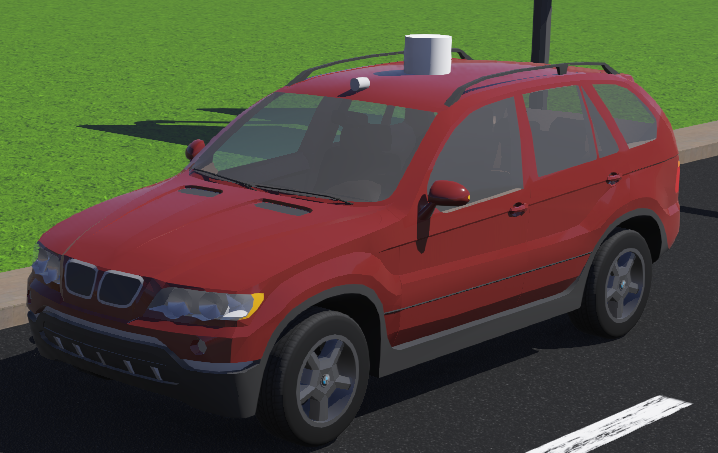
\includegraphics[width=\textwidth]{Figures/Figures_Cap03/test_car.png}
         \caption{Vehículo de pruebas instrumentado con sensores.}
         \label{fig:webots_car}
     \end{subfigure}
     
    \caption{Escenario y vehículo de pruebas.}
    \label{fig:world_car_test}
\end{figure}

En lo que respecta al vehículo de pruebas Webots incluye modelos de vehículos populares, estos modelos tienen características muy generales como, luces, llantas, tipo de motor, retrovisores, color y otros elementos comunes de un vehículo. Lo importante a destacar es que cada vehículo cuenta con secciones predefinidas para instrumentar el vehículo con los sensores necesarios. Para los propósitos de este proyecto se utiliza un vehículo 'X5' de 'BMW' en color rojo. A este vehículo se le añaden los siguientes sensores:
\begin{itemize}
    \item Cámara RGB, colocada en la parte frontal del vehículo.
    \item Lidar, colocado en la parte superior del vehículo.
    \item GPS, colocado en la parte frontal y superior del vehículo.
\end{itemize}

El vehículo para pruebas de navegación instrumentado con los sensores y actuadores necesarios se encuentra ilustrado en la figura \ref{fig:webots_car}.

Es es importante mencionar que el vehículo de pruebas 'BMW X5' es manipulado a través de un controlador, este se encarga de recibir información de cada sensor. Además, el mismo controlador envía señales para el control de velocidad, ángulo de dirección entre otros. En los próximos capítulos se ofrece una descripción con mayor detalle de cada uno de los nodos utilizados. En cuanto a los vehículos en movimiento dentro de la carretera se emplea un controlador supervisor para manipular la posición y velocidad de los vehículos.

\section{Contribuciones en el TMR} \label{sec:contribuciones_en_el_TMR}

El ambiente de simulación y vehículo de pruebas instrumentado fueron de ayuda en el desarrollo de la plataforma de uso para las pruebas consideradas en el TMR- AutoModelCar 2022 en su modalidad virtual. El uso de este simulador permitió generar los ambientes de simulación para las pruebas de:
\begin{itemize}
    \item Navegación autónoma sin obstáculos.
    \item Navegación autónoma con obstáculos estáticos.
    \item Navegación autónoma con obstáculos dinámicos.
    \item Estacionamiento autónomo.
\end{itemize}
Con ayuda del desarrollo de controladores supervisores se logró el control de posición y velocidad de los diferentes autos que actuaron como obstáculo en cada prueba. El desarrollo del controlador principal del vehículo de pruebas permitió el control de movimiento del mismo en base a los sensores integrados.
\\
\\

% CONCLUSIONES DEL CAPÍTULO
Al termino de este capítulo se entienden los conceptos básicos, ventajas y desventajas del simulador Webots. Además, se conoce el enfoque que se le dará al entorno de simulación en la búsqueda de implementar y probar algoritmos de navegación autónoma. Los escenarios modelados así como el vehículo de pruebas instrumentado en este capítulo son parte esencial en los capítulos siguientes, pues permitirán evaluar el desempeño de los algoritmos desarrollados y el comportamiento del vehículo en las diferentes situaciones que se le presenten.